% !TEX TS-program = pdflatex
% !TEX encoding = UTF-8 Unicode

% This is a simple template for a LaTeX document using the "article" class.
% See "book", "report", "letter" for other types of document.

\documentclass[20pt]{article} % use larger type; default would be 10pt

\usepackage[utf8]{inputenc} % set input encoding (not needed with XeLaTeX)

%%% Examples of Article customizations
% These packages are optional, depending whether you want the features they provide.
% See the LaTeX Companion or other references for full information.

%%% PAGE DIMENSIONS
\usepackage{geometry} % to change the page dimensions
\geometry{a4paper} % or letterpaper (US) or a5paper or....
% \geometry{margin=2in} % for example, change the margins to 2 inches all round
% \geometry{landscape} % set up the page for landscape
%   read geometry.pdf for detailed page layout information

\usepackage{graphicx} % support the \includegraphics command and options

% \usepackage[parfill]{parskip} % Activate to begin paragraphs with an empty line rather than an indent

%%% PACKAGES
\usepackage{booktabs} % for much better looking tables
\usepackage{array} % for better arrays (eg matrices) in maths
\usepackage{paralist} % very flexible & customisable lists (eg. enumerate/itemize, etc.)
\usepackage{verbatim} % adds environment for commenting out blocks of text & for better verbatim
%\usepackage{subfig} % make it possible to include more than one captioned figure/table in a single float
\usepackage{mathtools}
\usepackage{graphicx} % supports images in latex
% These packages are all incorporated in the memoir class to one degree or another...

\usepackage{graphicx}
\usepackage{subcaption}

%%% Other stuff
\DeclarePairedDelimiter\ceil{\lceil}{\rceil}
\DeclarePairedDelimiter\floor{\lfloor}{\rfloor}

%%% HEADERS & FOOTERS
\usepackage{fancyhdr} % This should be set AFTER setting up the page geometry
\pagestyle{fancy} % options: empty , plain , fancy
\renewcommand{\headrulewidth}{0pt} % customise the layout...
\lhead{}\chead{}\rhead{}
\lfoot{}\cfoot{\thepage}\rfoot{}

%%% SECTION TITLE APPEARANCE
\usepackage{sectsty}
\allsectionsfont{\sffamily\mdseries\upshape} % (See the fntguide.pdf for font help)
% (This matches ConTeXt defaults)

%%% ToC (table of contents) APPEARANCE
\usepackage[nottoc,notlof,notlot]{tocbibind} % Put the bibliography in the ToC
\usepackage[titles,subfigure]{tocloft} % Alter the style of the Table of Contents
\renewcommand{\cftsecfont}{\rmfamily\mdseries\upshape}
\renewcommand{\cftsecpagefont}{\rmfamily\mdseries\upshape} % No bold!

%%% graphics path
\usepackage{amsmath}
\usepackage{listings}
%\begin{lstlisting}[language=java]
%\end{lstlisting}



%%% END Article customizations

%%% nice things to keep around
%\begin{figure}[!htbp]
%  	\centering
%   	\begin{subfigure}[p]{0.5\linewidth}
%    	\includegraphics[width=\linewidth]{}
%   	\end{subfigure}
%\end{figure} 

% \noindent\rule{2cm}{0.4pt} 
%%% puts a small horizontal line

% \mathcal{O} 
%%% big O notation

% \begin{table}[!htbp]
% \caption{Forward slash.}
% \[\begin{array}{c|ccccc} 
% abc/def & 1 & 2 & 3 & 4 & 5\\
% \hline
% 1 & a & b & c & d & e\\
% 2 & f & g & h & i & j\\
% 3 & k & l & m & n & o\\
% \end{array}\]
% \end{table}

%%% The "real" document content comes below...

\title{Computational Statistics Midterm}
\author{Liam Dillingham}
%\date{} % Activate to display a given date or no date (if empty),
         % otherwise the current date is printed 

\begin{document}
\maketitle

\section{Problem 1}
Derive any one scheme for drawing samples from the diamond shaped area:\\
\noindent\rule{2cm}{0.4pt} \\
The R code for this is shown below:
\begin{lstlisting}[language=R]
arfunction = function() {
  while(TRUE) {
    x = runif(1,min = -1,max = 1)
    y = runif(1,min = -1, max = 1)
    if (abs(x) + abs(y) <= 1){
      rv = c(x, y)
      return(rv)
    }
  }
}
samples = matrix(nrow = 3000, ncol = 2)
for(i in 1:3000) {
  x = arfunction()
  samples[i,1] = x[1]
  samples[i,2] = x[2]
}
plot(samples[,1],samples[,2])
\end{lstlisting}
And the corresponding plot: 
\begin{figure}[!htbp]
  	\centering
   	\begin{subfigure}[p]{0.55\linewidth}
    	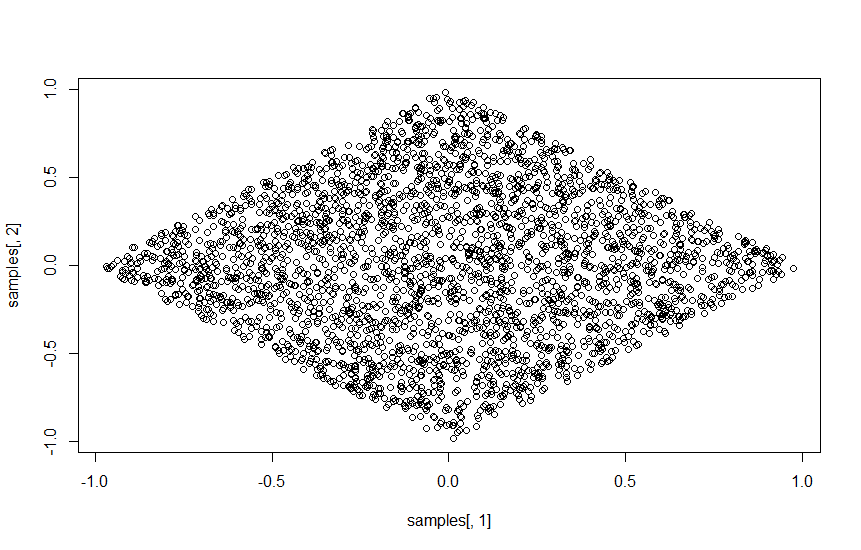
\includegraphics[width=\linewidth]{../figures/midterm1.png}
   	\end{subfigure}
\end{figure} 
\newpage
\section{Problem 2}
It is well-known that ridge regression tends to give similar coefficient values to correlated variables, whereas the lasso may give quite different coefficient values to correlated vari-ables. We will now explore this property in a very simple setting.\\
Suppose that $n = 2, p = 2, x_{11} = x_{12}, x_{21} =x_{22}$. Furthermore, suppose that $y_1 + y_2 = 0$, $x_{12}+x_{22}=0$, and $x_{11} + x_{21} = 0$, so that the estimate for the intercept in a least squares, ridge regression, or lasso model is zero: $\hat{\beta_0} = 0$.
\subsection{Write out the ridge regression optimization problem in this setting}
I'm trying to visualize the problem at hand here. We have a system that looks like this:
$$\begin{bmatrix} 
x_{11} & x_{12}\\
x_{21} & x_{22} 
\end{bmatrix}
\begin{bmatrix} 
\hat{\beta_1}\\
\hat{\beta_2}
\end{bmatrix}
=
\begin{bmatrix} 
y_1\\
y_2
\end{bmatrix}
$$
So we want to find the values of the $\hat{\beta_i}$'s in the equation $x_{i1}\hat{\beta_1} + x_{i2}\hat{\beta_2} = \hat{y_i}$ such that the computed value, $(\hat{y_i}-y_i)^{2}$ is minimized for all $i$.  In our $p = 2$ case, we want to minimize $(\hat{y_1}-y_1)^{2} + (\hat{y_2}-y_2)^{2}$.  However, since we are performing ridge regression, we alter this equation such that we are minimizing the equation:
$$(y_1 - (m_i x_{1i} + b_i)^{2} + (y_2 - (m_1 x_{2i} + b_i))^{2} + \lambda m_i^{2}$$
For each $i \in p=2$. By doing some algebra, we rearrange the equation to:
$$(y_1^{2} + y_2^{2}) - 2 m_i(x_{1i} y_1 + x_{2i} y_2) - 2 b_i(y_1+y_2) + m_i^{2}(x_{1i}^{2} + x_{2i}^{2}) + 2 m_i b_i (x_{1i} + x_{2i}) + 2b_i^{2} + \lambda m_1^{2}$$
Since $\overline{x_i} = \frac{ x_1 + x_2 + ... + x_n}{n}$, and in this case, $n = p = 2$, then $\overline{x_i} = \frac{x_1 + x_2}{2}$, or $x_1 + x_2 = 2\overline{x_i}$.  So we can replace a few of these terms:
$$2\overline{y^{2}} - 4m_i\overline{x_iy} - 4b_i\overline{y} + 2m_i^{2}\overline{x_i^{2}} + 4m_ib_i\overline{x_i} + 2b_i^{2} + \lambda m_i^{2}$$
To find the line of best fit, we want to find the minimum point on the error surface produced by $m$ and $b$.  We can find those values by calculating the partial derivates for $m$ and $b$, and setting them equal to 0.
$$\frac{\partial SSE}{\partial m_i} = -4\overline{x_iy} + 4m_i\overline{x_i^{2}} + 4b_i\overline{x_i} + 2 \lambda m_i = 0$$
$$\frac{\partial SSE}{\partial b_i} = -4\overline{y} + 4 m_i \overline{x_i} + 4b_i = 0$$
We want to coerce these equations into a $y=mx+b$ form, so we do some more algebraic manipulation:
$$\frac{\partial SSE}{\partial m_i} = m_i (\frac{4 \overline{x_i^{2}} + 2 \lambda}{4 \overline{x_i}}) + b_i = \frac{\overline{x_iy}}{\overline{x_i}} = 0$$
$$\frac{\partial SSE}{\partial b_i} = m_i \overline{x_i} + b_i = \overline{y} = 0$$
\newpage
And then we have a system of equations, and we can solve for $m$ and $b$. we multiply the partial derivative with respect to $m$ by -1, and add it to the other equation:
$$m_i ( \overline{x_i} - \frac{4 \overline{x_i^{2}} + 2 \lambda}{4 \overline{x_i}}) = \overline{y} - \frac{\overline{x_i y}}{\overline{x_i}}$$
Then, to isolate $m_i$, we divide both sides by its coefficient and simplify:
$$m_i = \frac{4 \overline{y} \ \overline{x_i} - \overline{x_i y}}{4( \overline{x_i} )^{2} - 4 \overline{x_i^{2}} + 2 \lambda}$$
And to solve for $b_i$ we substitute back into the equation and solve: $m_i \overline{x_i} + b_i = \overline{y} \Rightarrow b_i = \overline{y} - m_i \overline{x_i}$.
$$b_i = \overline{y} - \frac{4 \overline{y} \ \overline{x_i} - \overline{x_i y}}{4( \overline{x_i} )^{2} - 4 \overline{x_i^{2}} + 2 \lambda} \ \overline{x_i} 
= \overline{y} - \frac{4 \overline{y} \ (\overline{x_i})^{2} - \overline{x_i y} \ \overline{x_i}}{4( \overline{x_i} )^{2} - 4 \overline{x_i^{2}} + 2 \lambda}$$

Now, it is worth noting a few key facts about this problem. Since $y_1 + y_2 = 0$, $x_{12}+x_{22}=0$, and $x_{11} + x_{21} = 0$, then $x_{1i} + x_{2i} = 0$, for all $i$. Thus $\overline{x_i} = 0$. So we can eliminate a few terms.
$$m_i = \frac{4 \overline{y} \ 0 - \overline{x_i y}}{4( 0 )^{2} - 4 \overline{x_i^{2}} + 2 \lambda} = \frac{- \overline{x_i y}}{ - 4 \overline{x_i^{2}} + 2 \lambda}$$
$$b_i = 0 - \frac{0 - \overline{x_i y} \ 0}{4( 0 )^{2} - 4 \overline{x_i^{2}} + 2 \lambda} = 0$$



\subsection{Argue that in this setting, the ridge coefficient estimates satisfy $\hat{\beta_1} = \hat{\beta_2}$.}
note that $x_{11} = x_{12}, x_{21} =x_{22}$. Since $b_i = 0$ for all $i$, then we don't need to calcualte $b$. However, let's calculate $m_1$. \\
$- \overline{x_1 y} = \frac{1}{2}(x_{11}y_1 + x_{21}y_2)$, and $\overline{x_1^{2}} = \frac{1}{2}(x_{11}^{2} + x_{21}^{2})$. So,
$$m_1 = \frac{-\frac{1}{2}(x_{11}y_1 + x_{21}y_2)}{-2 (x_{11}^{2} + x_{21}^{2}) + 2 \lambda} \ \ \text{and likewise, }$$
$$m_2 = \frac{-\frac{1}{2}(x_{12}y_1 + x_{22}y_2)}{-2 (x_{12}^{2} + x_{22}^{2}) + 2 \lambda}$$
using the identities $x_{11} = x_{12}, x_{21} =x_{22}$ in the equation for $m_2$,
$$m_2 = \frac{-\frac{1}{2}(x_{11}y_1 + x_{21}y_2)}{-2 (x_{11}^{2} + x_{21}^{2}) + 2 \lambda} = m_1$$
Using the notation $\hat{\beta_1} = m_1$ and $\hat{\beta_2} = m_2$, we have satisfied $\hat{\beta_1} = \hat{\beta_2}$.

\newpage
\subsection{Write out the lasso optimzation problem in this setting.}
Note that for lasso regression, instead of penalizing the SSE by $\lambda m_i^{2}$, we penalize it by $\lambda |m_i|$.  We can actually skip a few of the initial steps of the previous problem, since the differences begin at derivation.  Note that instead of differentiating $m_i^{2}$, we differentiate $|m_i|$, where $\frac{\partial SSE}{\partial m_i} = \frac{m_i}{|m_i|}$. Starting with our original equation adjusted for lasso regression:
$$2\overline{y^{2}} - 4m_i\overline{x_iy} - 4b_i\overline{y} + 2m_i^{2}\overline{x_i^{2}} + 4m_ib_i\overline{x_i} + 2b_i^{2} + \lambda |m_i|$$
We then take the partial derivatives:
$$\frac{\partial SSE}{\partial m_i} = -4\overline{x_iy} + 4m_i\overline{x_i^{2}} + 4b_i\overline{x_i} +  \lambda \frac{m_i}{|m_i|} = 0$$
$$\frac{\partial SSE}{\partial b_i} = -4\overline{y} + 4 m_i \overline{x_i} + 4b_i = 0$$
However, due to the absolute value of $m_i$, we will be breaking this equation down into two cases, $m_i = m_i$ when $m_i \geq 0$, and $m_i = -m_i$ when $m_i < 0$.  And again, coercing the equations into our $mx+b$ form: \\
\textit{Case 1: $m_i < 0$}
$$\frac{\partial SSE}{\partial m_i} = -4\overline{x_iy} + 4m_i\overline{x_i^{2}} + 4b_i\overline{x_i} +  \lambda \frac{m_i}{-m_i} = 0$$
$$\frac{\partial SSE}{\partial m_i} =m_i \frac{\overline{x_i^{2}}}{\overline{x_i}} + b_i =  \frac{\overline{x_iy}}{\overline{x_i}} +  \frac{1}{4}\lambda \ \ \text{And for } b_i,$$
$$\frac{\partial SSE}{\partial b_i} = m_i \overline{x_i} + b_i = \overline{y} = 0$$
We multiply the equation for $m_i$ by -1, add the two equations together, and simplify
$$m_i = \frac{ \overline{x_i} \ \overline{y} - \overline{x_iy} - \frac{\lambda}{4}}{( \overline{x_i} )^{2} - \overline{x_i^{2}}}$$
Let's first simplify this equation further with the previously known fact that $\overline{x_i} = 0$.
$$m_i = \frac{- \overline{x_iy} - \frac{\lambda}{4}}{- \overline{x_i^{2}}} \ \ \text{ then } b_i \text{ equals: }$$
$$b_i = \frac{- \overline{x_iy} - \frac{\lambda}{4}}{- \overline{x_i^{2}}} \ 0 + b_i = 0 \ \text{, Since we already know } \overline{x_i} \text{ and } \overline{y_i} = 0$$
now for case 2. \\
\textit{Case 2: $m_i \geq 0$}
$$\frac{\partial SSE}{\partial m_i} = -4\overline{x_iy} + 4m_i\overline{x_i^{2}} + 4b_i\overline{x_i} +  \lambda \frac{m_i}{m_i} = 0$$
$$\frac{\partial SSE}{\partial m_i} =m_i \frac{\overline{x_i^{2}}}{\overline{x_i}} + b_i =  \frac{\overline{x_iy}}{\overline{x_i}} -  \frac{1}{4}\lambda \ \ \text{And for } b_i,$$
$$\frac{\partial SSE}{\partial b_i} = m_i \overline{x_i} + b_i = \overline{y} = 0$$
The situation is very similar. We can already infer that $b_i = 0$, due to the multiplication from the fact that $\overline{x_i} \text{ and } \overline{y_i} = 0$. Thus,
$$m_i = \frac{- \overline{x_iy} + \frac{\lambda}{4}}{- \overline{x_i^{2}}}$$
\subsection{Argue that in this setting, the lasso coefficients $\hat{\beta_1}$ and $\hat{\beta_2}$ are not unique - in other words, there are many possible solutions to the optimization problem in $(3)$. Describe these solutions.}
The values for the two $\hat{\beta_1}$ and $\hat{\beta_2}$

\section{Problem 3}
A study on the metabolism in 15-year-old females yielded the following data:
$x = (91, 504, 557, 609, 693, 727, 764, 803, 857, 929, 970, 1043, 1089, 1195, 1384, 1713)$.  Their energy intake in megajoules, follows a joint density.
\subsection{Prove the full conditional distributions of $\theta$ and $\sigma^{2}$}
Using the provided full condition, we derive the necessary conditional distributions:
$$f(\sigma^{2} \mid x, \theta) = \Bigg[ \frac{1}{(\sigma^{2})^{n/2}}exp\Bigg( -\Sigma_i (x_i - \theta)^{2} / (2\sigma^{2}) \Bigg) \Bigg] \times \Bigg[ \frac{1}{\tau} exp \Bigg( -(\theta - \theta_0)^{2} / (2\tau^{2}) \Bigg) \Bigg] \times \Bigg[ \frac{1}{(\sigma^{2})^{a+1}}exp\Bigg( \frac{-b}{\sigma^{2}} \Bigg) \Bigg]$$
Starting with deriving $\sigma^{2} \mid x, \theta$:
$$f(\sigma^{2} \mid x, \theta) = \Bigg[ \frac{1}{(\sigma^{2})^{n/2}}exp\Bigg( -\Sigma_i (x_i - \theta)^{2} / (2\sigma^{2}) \Bigg) \Bigg] \times \Bigg[ \frac{1}{(\sigma^{2})^{a+1}}exp\Bigg( \frac{-b}{\sigma^{2}} \Bigg) \Bigg] \ \text{ and rearrange:}$$
$$f(\sigma^{2} \mid x, \theta)= \Bigg[ \frac{1}{(\sigma^{2})^{n/2}} \frac{1}{(\sigma^{2})^{a+1}}exp\Bigg( -\Sigma_i (x_i - \theta)^{2} / (2\sigma^{2}) \ \frac{-b}{\sigma^{2}} \Bigg) \Bigg]$$
$$f(\sigma^{2} \mid x, \theta)= \Bigg[ \frac{1}{(\sigma^{2})^{n/2 + a + 1}} exp\Bigg( -\Sigma_i (x_i - \theta)^{2} / (2\sigma^{2}) \ \frac{-b}{\sigma^{2}} \Bigg) \Bigg]$$
$$f(\sigma^{2} \mid x, \theta)= \Bigg[ \frac{1}{(\sigma^{2})^{n/2 + a + 1}} exp\Bigg( - \Bigg( \frac{1}{2} \frac{\Sigma_i (x_i - \theta)^{2}}{\sigma^{2}} + \frac{b}{\sigma^{2}} \Bigg) \Bigg) \Bigg]$$
Thus the parameters of $\sigma^{2} \mid x, \theta$ have the form $a = n/2 + a$ and $b = \frac{1}{2} \Sigma_i (x_i - \theta)^{2} + b$. Next, we prove the conditional for $\theta \mid x, \sigma^{2}$:
$$f(\theta \mid x, \sigma^{2}) = \Bigg[ \frac{1}{(\sigma^{2})^{n/2}}exp\Bigg( -\Sigma_i (x_i - \theta)^{2} / (2\sigma^{2}) \Bigg) \Bigg] \times \Bigg[ \frac{1}{\tau} exp \Bigg( -(\theta - \theta_0)^{2} / (2\tau^{2}) \Bigg) \Bigg] \times \Bigg[ \frac{1}{(\sigma^{2})^{a+1}}exp\Bigg( \frac{-b}{\sigma^{2}} \Bigg) \Bigg]$$
$$f(\theta \mid x, \sigma^{2}) =  \frac{1}{(\sigma^{2})^{n/2 + a + 1}} exp \Bigg( \frac{-\Sigma_i (x_i - \theta)^{2}}{2\sigma^{2}} + \frac{-(\theta - \theta_0)^{2}}{2\tau^{2}}+\frac{-b}{\sigma^{2}} \Bigg)$$
By expanding the summation, we get: $(x_1^{2} + x_2^{2} + ... + x_n^{2}) + (-2\theta x_1 - 2\theta x_2 - ... - 2\theta x_n) + n\theta^{2}$.  Using the identity $n\overline{x} = x_1 + x_2 + ... + x_n$, we can remove the summation term from the equation:
$$=  \frac{1}{(\sigma^{2})^{n/2 + a + 1}} exp \Bigg( \frac{-2 \tau^{2} n ( \overline{x^{2}} - 2\theta \overline{x} + \theta^{2} ) + (2\sigma^{2})(-(\theta-\theta_0^{2})}{4\sigma^{2}\tau^{2}} + \frac{-b}{\sigma^{2}} \Bigg)$$
$$=  \frac{1}{(\sigma^{2})^{n/2 + a + 1}} exp \Bigg( \frac{-2 \tau^{2} n ( \overline{x^{2}} - 2\theta \overline{x} + \theta^{2} ) + (-2\sigma^{2})( \theta^{2}-2\theta \theta_0+\theta_0^{2} )}{4\sigma^{2}\tau^{2}} + \frac{-b}{\sigma^{2}} \Bigg)$$

\subsection{Using the normal model above, implement the gibbs sampler}
\begin{lstlisting}[language=R]
x = c(91, 504, 557, 609, 693, 727, 764, 803, 857, 
	929, 970, 1043, 1089, 1195, 1384, 1713)
n = length(x)
a = 3
b = 3
tau2 = 10
theta0 = 5

theta_mu = function(sig2) {
  mu1 = (sig2 * theta0) / (sig2 + n * tau2)
  mu2 = (n * tau2 * mean(x)) / (sig2 + n * tau2)
  return(mu1 + mu2)
}

theta_sig = function(sig2) {
  sig = (sig2 * tau2) / (sig2 + n * tau2)
  return(sig)
}

gibbs <- function(burn = 1000, nmc = 2000){
  
  theta <- rep(0, nmc+burn)
  sigma2 <- rep(0, nmc+burn)
  
  sigma2[1] = rinvgamma(1, (n/2) + a, 0.5 * sum((x - theta0)^(2)) + b)
  theta[1] = theta0; 
  
  for (i in 2:(burn+nmc)) {
    
    sigma2[i] <- rinvgamma(1, (n/2) + a, theta[i-1])
    theta[i] <- rnorm(1, theta_mu(sigma2[i]), theta_sig(sigma2[i]))
  }
  return(list(sigma2=sigma2,theta=theta))
}
\end{lstlisting}
\subsection{Plot histograms of $\log(\theta)$ and $\log(\sigma^{2})$ and report $90\%$ posterior probability intervals for both}
\begin{figure}[!htbp]
  	\centering
   	\begin{subfigure}[p]{0.7\linewidth}
    	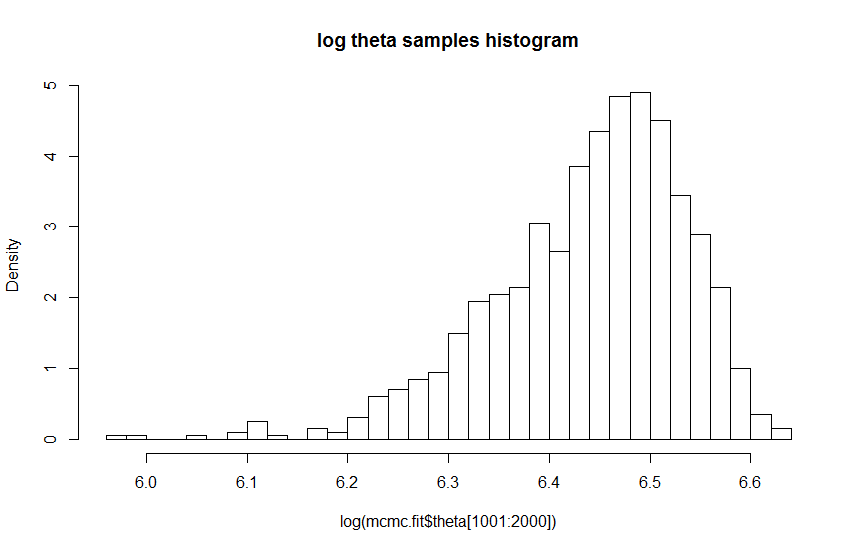
\includegraphics[width=\linewidth]{../figures/midterm2.png}
   	\end{subfigure}
\end{figure} 
\begin{figure}[!htbp]
  	\centering
   	\begin{subfigure}[p]{0.7\linewidth}
    	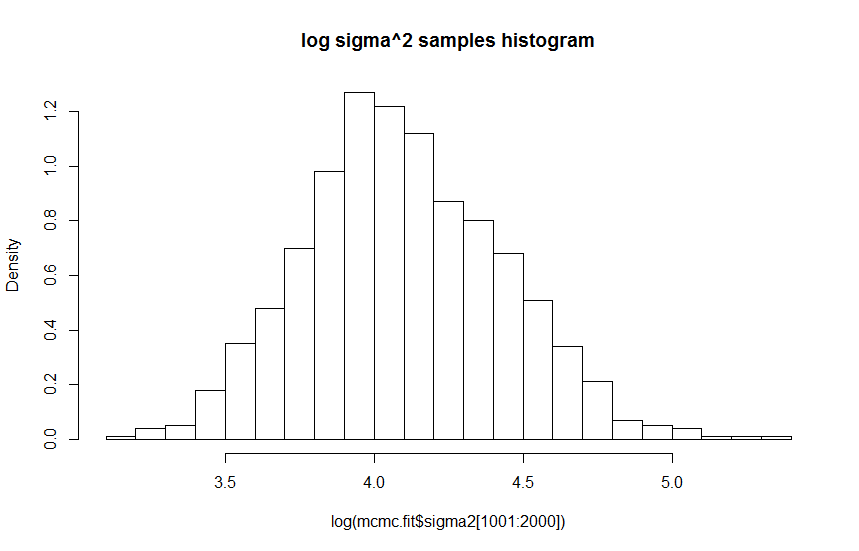
\includegraphics[width=\linewidth]{../figures/midterm3.png}
   	\end{subfigure}
\end{figure} 
\end{document}






































